\aufgabe 1

\paragraph{a)}\mbox{} \\

Das in der Aufgabe beschriebene Model ist als Typ LHA II des Linearen Hybrid Automaten unterzuordnen. Die Ableitungen von a und b sind dabei weder Konstanten oder Intervalle, welche dem Typen LHA I unterzuordnen wären. Es handelt stattdessen bei sämtlichen Ableitungen um Funktionen, welche zu nicht linearen Veränderungen über Zeit führen. 

\paragraph{b)}\mbox{} \\

Siehe die in der Abgabe beigelegte .xml-Datei. 

\paragraph{c)}\mbox{} \\

\begin{lstlisting}
	a==5000 &
	b==5000 &
	discharging\_rate==200 &
	charging\_rate==-100 &
	g==0 &
	min\_charge==10 &
	max\_charge==10 &
	min\_discharge==10 & 
	max\_discharge==10 &
	t\_charge==0 &
	t\_discharge==0 &
	loc(KineticBatteryModel\_1)==normal\_charging &
	loc(controller\_1)==charging 		
	
\end{lstlisting}


\paragraph{d)}\mbox{} \\

\begin{figure}[H]
	\centering
	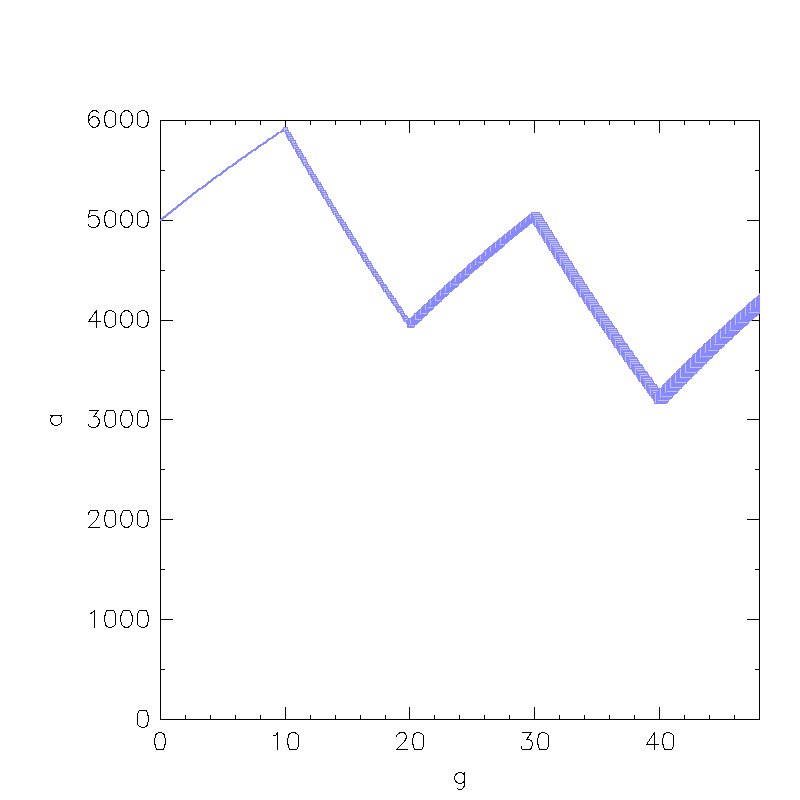
\includegraphics[width=0.55\textwidth]{Aufgabe_d).png}
\end{figure}	
	
In dieser Abbildung ist in den beginnenden 10 Stunden ein Ladevorgang in $a$ zu sehen. Sobald jedoch die Anforderung $a>b$ erfüllt ist, wird durch den Recovery Effect Ladung von $a$ an $b$ abgegeben. Aus diesem Grund ist nach 10 Stunden ein Abfall zu erkennen, wodurch $a$ nicht vollständig bis 6000 aufgeladen wird. \\


Ist die Anforderung $a>b$ im weiteren Verlauf erneut nicht erfüllt, kommt es zu einer Umkehrung des Recovery Effects, wodurch $a$ erneut aufgeladen wird. Dieser Vorgang wechselt sich entsprechend ab und es kommt zu Wiederholungen, wie an dem Auf- und Abstieg von $a$ im obigen Graphen zu sehen ist. \\


Die in der Grafik größer werdenden Polygone entstehen hier aufrgund einer Überapproximation seitens SpaceEx.


\paragraph{e)}\mbox{} \\

\begin{figure}[H]
	\centering
	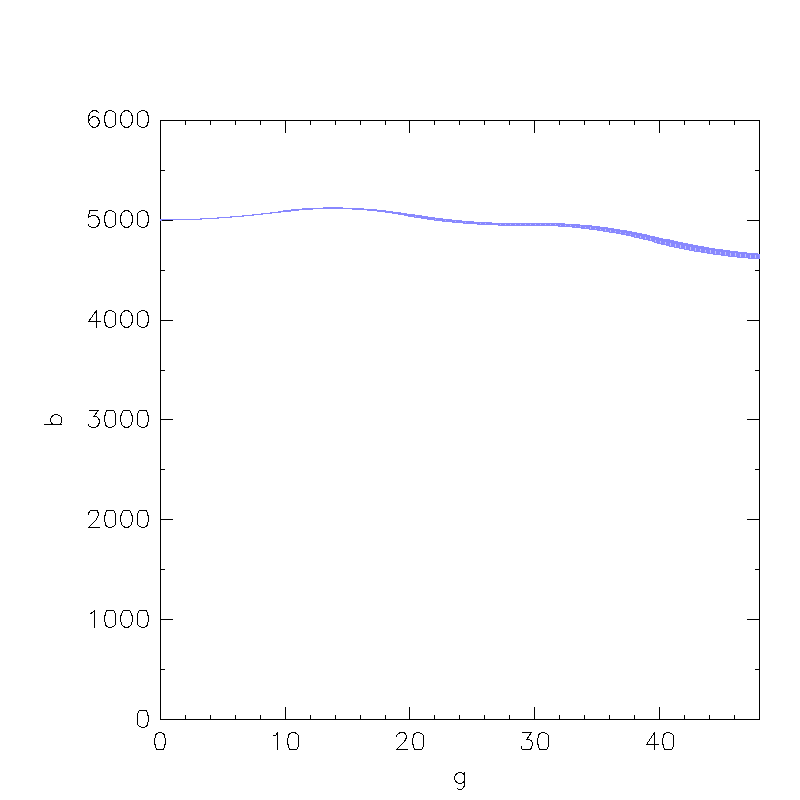
\includegraphics[width=0.55\textwidth]{Aufgabe_e).png}
\end{figure}

Wie schon in Aufgabe d) zu erkennen war, ist auch in diesem Graphen der Recovery Effect widergespiegelt. Je größer der Abstand zu $a$ wird umso stärker wird dieser Effekt. Durch die Anforderung $a>b$ wird $b$ weiterhin im dem Punkt geladen indem a bereits entladen ist. Der Graph hat weiterhin einen Scheitelpunkt sobald der Fall $a=b$ eintritt. Im Anschluss tritt der Fall $a<b$ ein, wodurch Ladung von $b$ abgegeben wird. Analog zur vorherigen Aufgabe wiederholt sich der Vorgang. 


Auch in diesem sowie dem darauffolgenden Graphen ist eine Überapproximation zu sehen. 
\newpage

\paragraph{f)}\mbox{} \\

\begin{figure}[H]
	\centering
	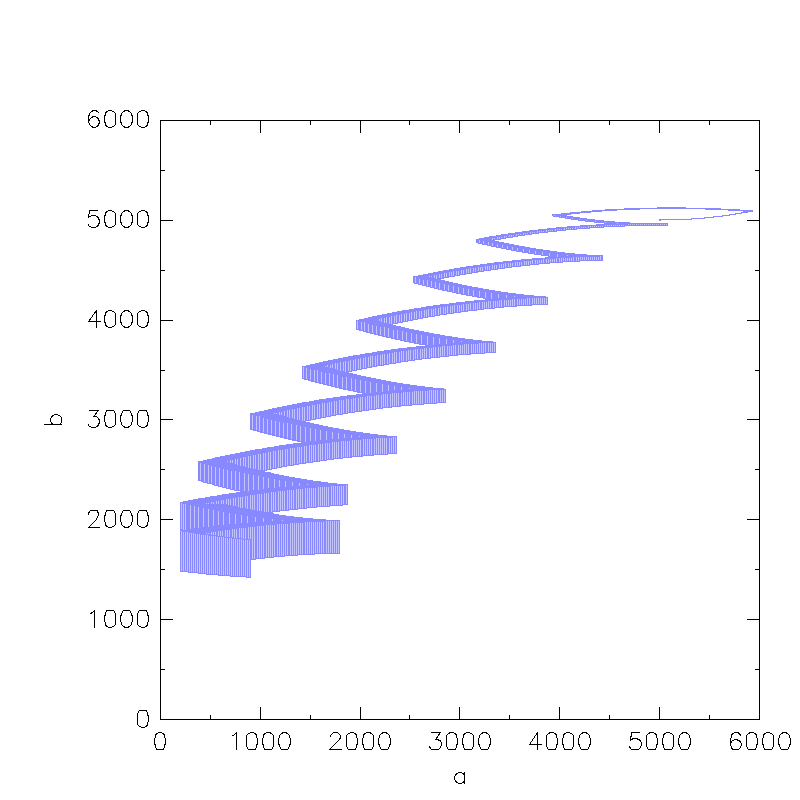
\includegraphics[width=0.555\textwidth]{Aufgabe_f).png}
\end{figure} 

Wie bereits erwartet ist eine Kombination des Graphenverlaufs von d) und e) zu erkennen. Zunächst ist ein Anstieg von $a$ und $b$ zu erkennen. Sobald 10 Stunden vergangen sind und $a>b$ erfüllt wird, fällt $a$ ab und $b$ steigt weiterhin an. 

Sobald $a=b$ erreicht ist, beginnt auch $b$ zu fallen. 

Insgesamt nimmt die Ladung ab, da die Entladungsrate höher ist, als die Rate der Ladung.


\paragraph{g)}\mbox{} \\
\begin{minipage}[t]{0.5\textwidth} 
	\begin{figure}[H]
		\centering
		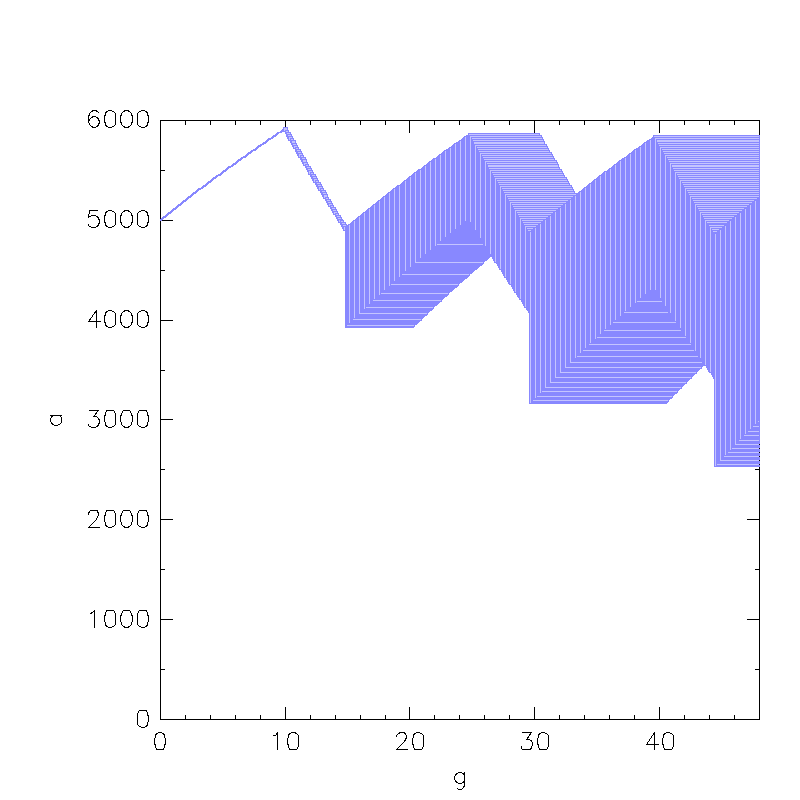
\includegraphics[width=0.8\textwidth]{Aufgabe_g1).png}
	\end{figure}
\end{minipage}
\hfill
\begin{minipage}[t]{0.5\textwidth} 
	\begin{figure}[H]
		\centering
		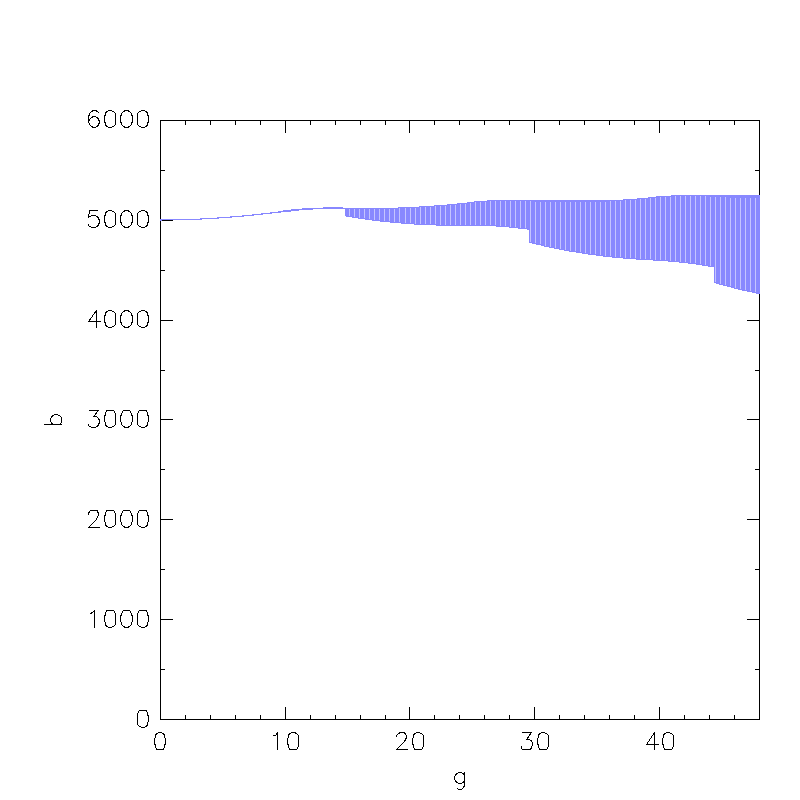
\includegraphics[width=0.8\textwidth]{Aufgabe_g2).png}
	\end{figure}
\end{minipage}\\ 

Im Vergleich zu den vorherigen Graphen aus d) und e) ist hier erst eine Veränderung zwischen den Graphen ab der 15. Sekunde zu sehen. Aufgrund der veränderten Einstellung von $t_{\text{min\_discharge}}=5$ ist ein erneuter Charge-Vorgang bereits zu einem früheren Zeitpunkt möglich. Der Discharge-Vorgang kann somit eine Dauer von 5 bis 10 Stunden annehmen. Ist die Dauer des Discharge-Vorgangs hierbei minimal, erreicht $a$ im darauffolgenden Charge-Vorgang die Höhe, die vor dem Discharge-Vorgang erreicht wurde. Im Charge-Vorgang nach dem ersten Discharge wäre dies beispielsweise ein erneutes Aufladen bis zum lokalen Maxima. 

Ein Discharge-Vorgang mit maximaler Länge entspräche dabei weiterhin dem Verlauf von d) und e). 

Das hierdurch aufgespannte Spektrum von möglichen Ladungen von $a$ liefert somit eine größere Zustandsform. Diese ist in dem Graphen durch eine starke Überapproximation seitens SpaceEx zu erkennen. Die mit der Zeit größer werdenden Polygone spiegeln dabei sämtliche möglichen Ladungen von $a$ und $b$ wieder.
 

Das abwelchselnde Verhalten des Charge und Discharge-Vorgangs bleibt jedoch weiterhin erhalten, wie in den Graphen zu erkennen ist. 

\paragraph{h)}\mbox{} \\

%\begin{minipage}[t]{0.5\textwidth} 
%	\begin{figure}[H]
%		\centering
%		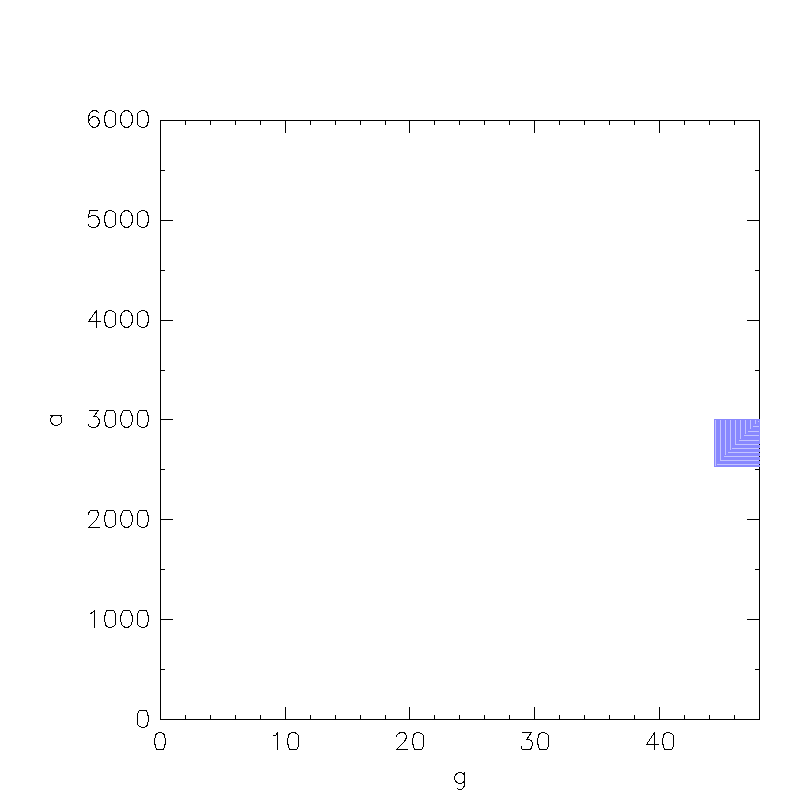
\includegraphics[width=0.8\textwidth]{Aufgabe_h1).png}
%	\end{figure}
%\end{minipage}
%\hfill
%\begin{minipage}[t]{0.5\textwidth} 
%	\begin{figure}[H]
%		\centering
%		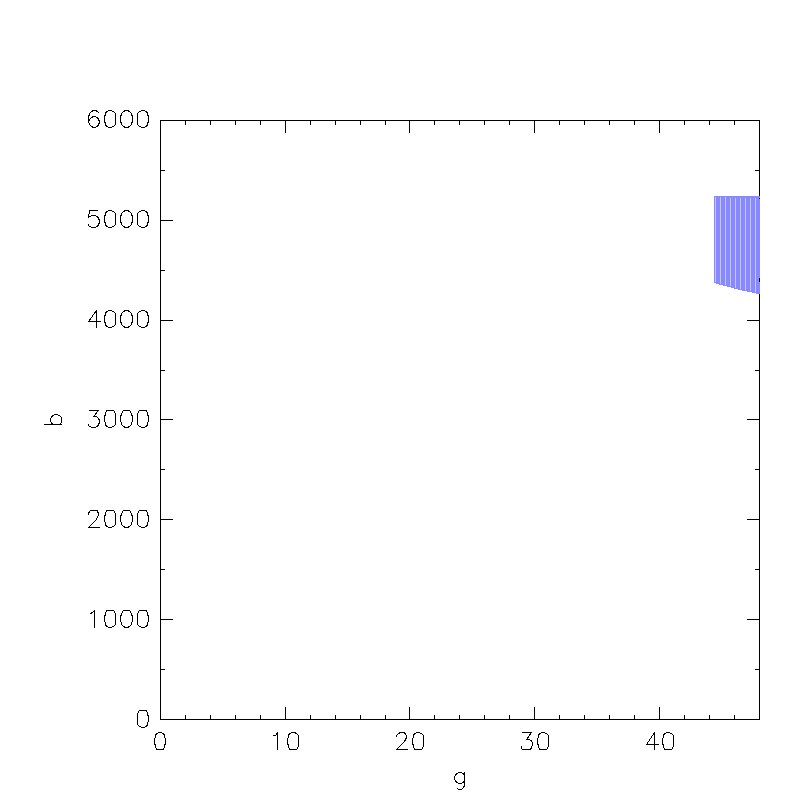
\includegraphics[width=0.8\textwidth]{Aufgabe_h2).png}
%	\end{figure}
%\end{minipage}
%\todo{Graph raus}


	
\begin{lstlisting}
Bounds on the variables over the entire set:

network.g: [44.4,181.8]
network.a: [26.3988,3000]

Location-wise bounds on the variables:

Location: loc(KineticBatteryModel_1)==normal_charging & 
loc(controller_1)==charging

network.g: [44.4,173.725]
network.a: [26.3988,3000]

Location: loc(KineticBatteryModel_1)==normal_discharging & 
loc(controller_1)==discharging

network.g: [46.8,181.8]
network.a: [200,3000]

Location: loc(KineticBatteryModel_1)==adapted_discharging & 
loc(controller_1)==discharging

network.g: [121.5,163.625]
network.a: [26.3988,200]

\end{lstlisting}

Wie schon in g) angemerkt dauert der maximale Discharge-Vorgang insgesamt 10 Stunden. Der schlimmste Entladungsfall tritt somit genau dann ein, wenn sämtliche durchgeführten Discharge-Vorgänge jeweils 10 Stunden andauern. 

Eine verfügbare Ladung, welche $< 3000$ mAh beträgt, ist somit bereits nach 44.4 Stunden möglich.


\paragraph{i)}\mbox{} \\

\begin{minipage}[t]{0.5\textwidth} 
	\begin{figure}[H]
		\centering
		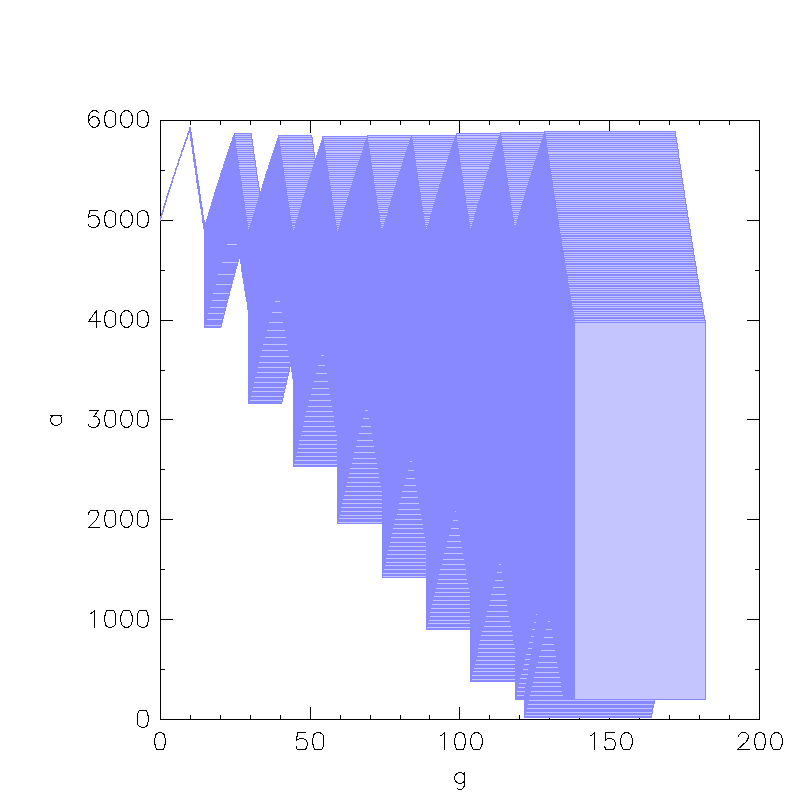
\includegraphics[width=0.8\textwidth]{Aufgabe_i1).png}
	\end{figure}
\end{minipage}
\hfill
\begin{minipage}[t]{0.5\textwidth} 
	\begin{figure}[H]
		\centering
		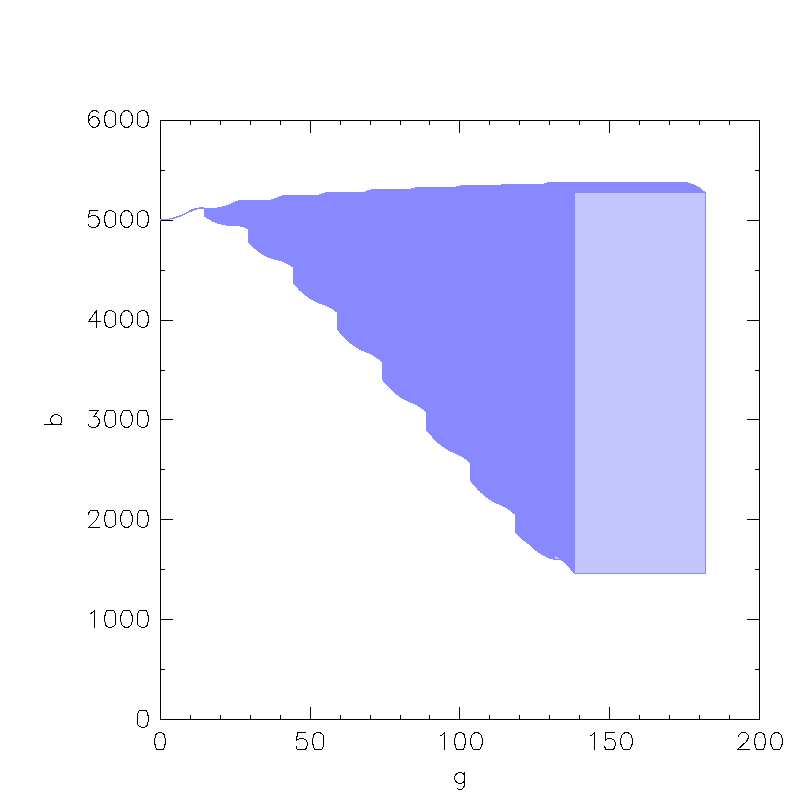
\includegraphics[width=0.8\textwidth]{Aufgabe_i2).png}
	\end{figure}
\end{minipage}\\ 

Auch hier kann es zu dem schlimmsten Entladungsfall von konstanten Discharge-Vorgängen à 10 Stunden kommen. Tritt dieser ein, wird mit gleicher Dauer auf- und abgeladen. Gleichzeitig findet der Discharge-Vorgang in der doppelten Geschwindigkeit statt, wodurch $a$ gegen 0 laufen und die Ladung somit leer werden kann.  

Da es weiterhin für $b$ nicht möglich ist vor $a$ entleert zu werden, kann es einen Zeitpunkt geben in dem $a$ leer und $b$ nicht leer ist. 

\paragraph{j)}\mbox{} \\

Wie in den darauffolgenden Graphen zu sehen ist, kann $a\leq 2500$ mAh nicht innerhalb von 48 Stunden erreicht werden.  \\
\begin{minipage}[t]{0.5\textwidth} 
	\begin{figure}[H]
		\centering
		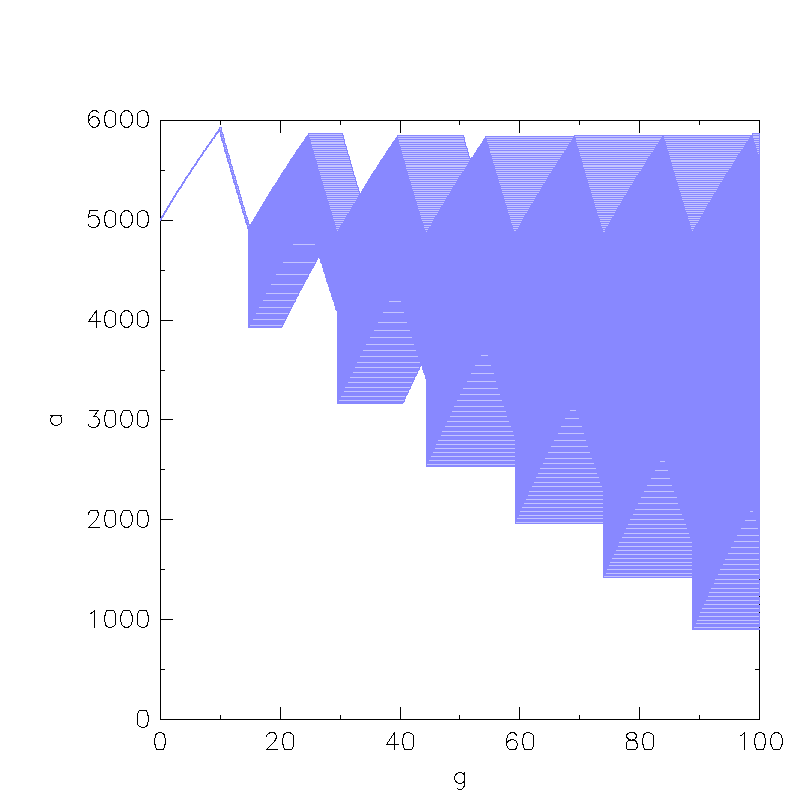
\includegraphics[width=0.8\textwidth]{Aufgabe_j1).png}
	\end{figure}
\end{minipage}
\hfill
\begin{minipage}[t]{0.5\textwidth} 
	\begin{figure}[H]
		\centering
		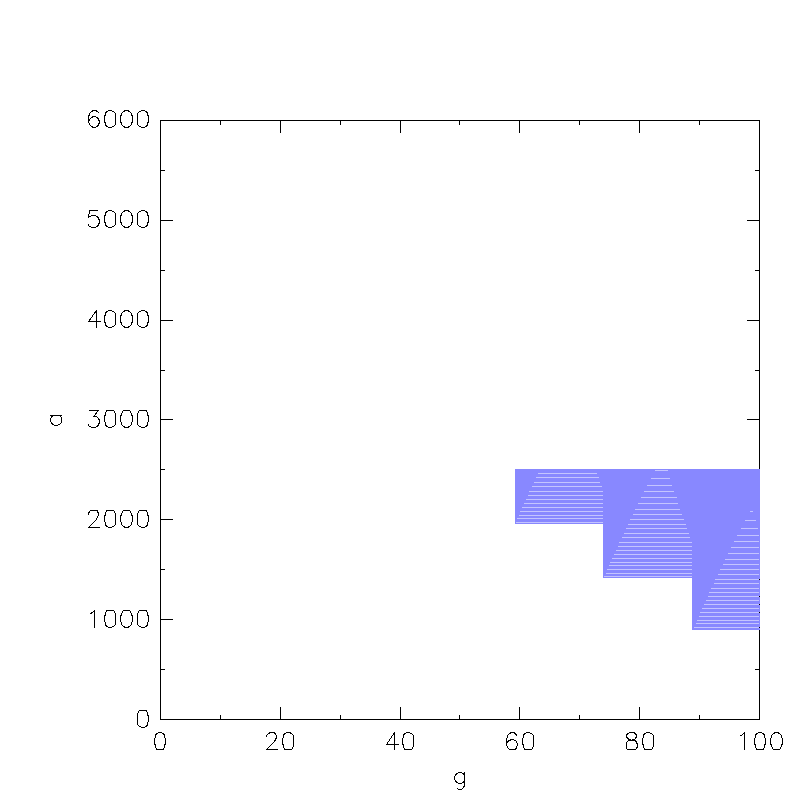
\includegraphics[width=0.8\textwidth]{Aufgabe_j2).png}
	\end{figure}
\end{minipage}

\paragraph{k)}\mbox{} \\

Es ist zu erkennen, dass $a$ mit einer leicht abfallenden Rate an Ladung dazugewinnt. 
Dies ist mit dem Recovery Effect zu erklären. 
Da zwischen $b$ und $a$ eine anfängliche Differenz von 3000 mAh besteht, gibt $b$ zu Beginn mehr Ladung ab. Im Anschluss pendeln sich die Ladungen von $a$ und $b$ mit abnehmender Geschwindigkeit in der Mitte von 2000 und 5000 mAh ein.

Dieses Verhalten ist im folgenden Graphen zu sehen:

\begin{figure}[H]
	\centering
	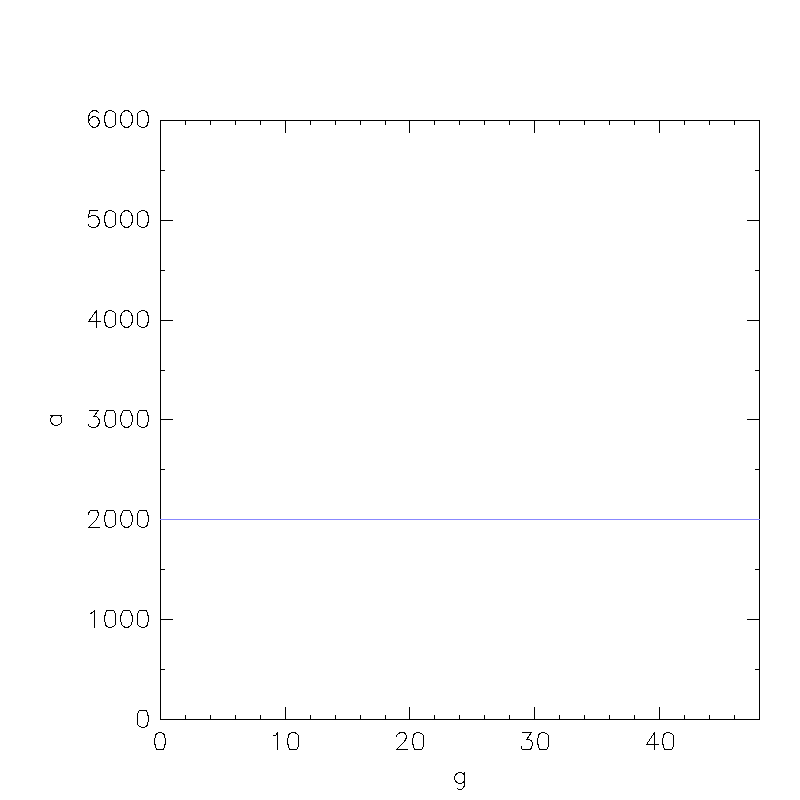
\includegraphics[width=0.55\textwidth]{Aufgabe_k).png}
\end{figure}